\begin{inprogress}
Researchers have been studying confinement for decades~\cite{lampson1973_confinement}, and
have been designing and applying confinement primitives since the early days of
time-sharing computers and multi-tenant systems~\cite{shu2016_security_isolation_study}.
Despite decades of research into the confinement problem, the status quo of confinement on
Linux, particularly from the perspective of containers, is in a sorry state. This chapter
outlines the difficulties that arise in the Linux confinement ecosystem due to its
inherent complexity, inflexible and interdependent components, and the difficulties that
arise in adopting newly-proposed alternatives. These insights represent the key
motivating factors behind the design of \bpfbox{} and \bpfcontain{} and can potentially
inform the way we think about new confinement mechanisms going forward.
\end{inprogress}

\section{Rethinking the Virtualization Narrative}%
\label{s:rethinking-virtualization}

Hypervisor-backed virtualization is commonly considered more secure than container-based
virtualization~\cite{sultan2019_container_security, eder2016_hypervisor_container}.
Intuitively, this makes sense. Containers run directly on the host operating system,
whereas a virtual machine runs on top of a hypervisor, separated by at least one layer of
indirection from the host system. However, this intuition does not strictly stand up to
scrutiny. A virtual machine running on top of a hypervisor makes requests to the
hypervisor's \gls{api} (via hypercalls), in much the same way as a container running on
a host operating system makes requests to the kernel's \gls{api} (via system calls).
\Cref{fig:syscall-hypercall} illustrates this parity.

\begin{figure}[htbp]
  \centering
  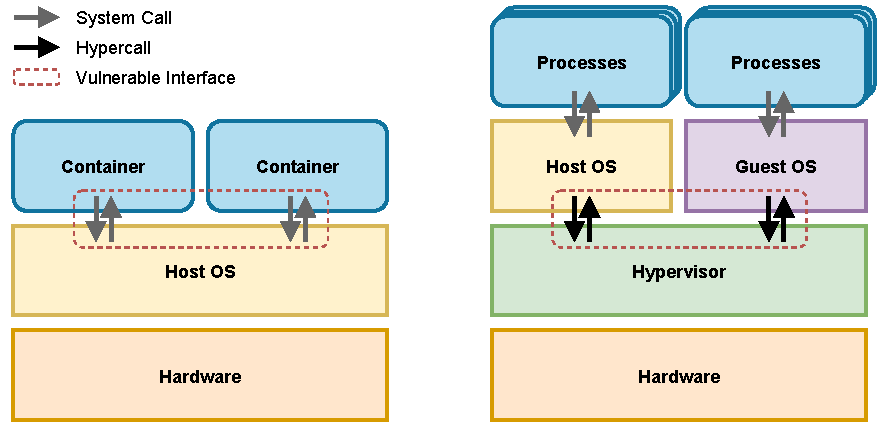
\includegraphics[width=0.8\linewidth]{figs/confinement-problem/syscall-hypercall.pdf}
  \caption[]{
    \todo{Caption here}
  }%
  \label{fig:syscall-hypercall}
\end{figure}

The isolation guarantees provided by a virtual machine come almost entirely from a sense
of obfuscation over a semantic gap, created as the hypervisor virtualizes system
resources. There is no notion of centralized policy in a virtual machine; rather, security
is an emergent phenomenon, a form of \enquote{policy through mechanism}. With the right
tools, we can and have poked holes everywhere in this
policy~\cite{dubrelle2015_hypervisor, thongthua2016_analysis, shahzad2017_systematic}.

The central argument of this thesis is that there is no fundamental reason why containers
cannot be as\,---\,if not more\,---\,secure than virtual machines.
\begin{inprogress}
  \begin{itemize}
    \item The point is that we just need to define a clear protection boundary
    \item \bpfbox{} lays the foundation for this, and \bpfcontain{} brings it home
    \item In \bpfbox{} policies are defined in a centralized, flexible policy file, and
          integrate a variety of possible behaviours together in a simple and clear way
    \item In \bpfcontain{}, we build a container abstraction into \bpfbox{}, and use this
          to inform an \textit{implicit policy}. This defines a very clear boundary for
          operations that can impact the container vs operations that can impact the system as
          a whole. Behaviour \textit{within} the container is unrestricted, whereas behaviour
          that can impact the world outside the container is implicitly denied. Policy then
          defines \textit{exceptions} to this implicit policy, rather than \textit{rules}.
    \item The key insight is that \gls{ebpf} allows us to get this container abstraction
          in a flexible and adoptable way, rather than forcing it into the mainline kernel.
          Yet we still have the flexibility to incorporate various aspects of system state
          into our enforcement decisions, beyond simple \gls{lsm} hooks.
  \end{itemize}
\end{inprogress}

\begin{inprogress}
  \begin{itemize}
    \item To accomplish something like this, we need a way to define a single, clear,
          protection boundary into containers
    \item This requires a fundamental change in the way containers are handled on the kernel side
    \item Specifically, we need a good abstraction for containers in order to be able to enforce
          a clear and effective policy for then
    \item Lead into the next section: Given the existing state of confinement on Linux,
          this may not seem like a feasible task, but we assert that new kernel technologies
          are making this possible (i.e.~eBPF and \bpfbox{}/\bpfcontain{}).
  \end{itemize}
\end{inprogress}

\begin{inprogress}
  \begin{itemize}
    \item Just like the word container makes people think about security
    \item Type I and Type II hypervisor, the way it's depicted, makes people think something else is happening
    \item The representation and terminology
    \item This makes sense to talk about it if we connect it to containers
    \item Why can't containers give as good or better security than hypervisors
    \item Can we just get our enforcement clear
    \item Virtual machines seem like they define a clear boundary, but it isn't actually
          so clear in practice because all these things are being shared across boundaries
    \item People think of virtual machines as being inherently more secure, the security
          benefit is more of an obfuscation thing related to the semantic gap but with the right
          tools you can still cross it freely
    \item VMs have all these little holes everywhere and the policy is not centralized\,---\,we
          have policy through mechanism
    \item There's no reason why containers can't be as (if not more) secure than virtual machines
    \item Because we can make this boundary very clear
    \item \bpfcontain{} can be seen as a step towards this
  \end{itemize}
\end{inprogress}

\section{Fundamental Issues with Linux Confinement}%
\label{s:cp-confinement-issues}

\begin{enumerate}
  \item \textbf{Complexity and Interdependence.}
    Existing confinement primitives are overly complex and designed for use
    cases beyond simple process confinement. This results in a pattern of
    abusing existing mechanisms
  \begin{inprogress}
    \begin{itemize}
      \item Existing confinement solutions are overly complex
      \item Based on a number of low-level primitives that were originally designed for
            totally different tasks.
      \item Namespaces were designed to virtualize resources. They provide a form of
            isolation but not confinement; need a way to deal with namespace escapes
      \item Cgroups, similarly, were designed to virtualize the availability of system
            resources, not to directly confine.
      \item Unix \gls{dac} is far too coarse-grained and easy to bypass to be practically useful for confinement.
      \item POSIX capabilities can be used to reduce overprivilege by portioning root privileges, but do not
            implement confinement by themselves.
      \item Seccomp-bpf works well to reduce the availability of system calls, but writing
            classic \gls{bpf} filters is complex and error-prone. Anything beyond basic system call
            filtering quickly becomes untenable, particularly considering race conditions when
            checking arguments.
    \end{itemize}
  \end{inprogress}

  \item \textbf{Inappropriate Defaults.}
  \begin{inprogress}
    \begin{itemize}
      \item
    \end{itemize}
  \end{inprogress}

  \item \textbf{Difficulty Adopting New Solutions.}
  \begin{inprogress}
    \begin{itemize}
      \item Motivated by the above difficulties, academics are often tempted to propose new confinement solutions.
      \item Many try to solve the problem by simply recombining and reusing these existing primitives in new ways.
      \item This isn't really a step forward, as we are still subject to limitations introduced in item 1 and item 2.
      \item To really solve the problem, we need kernel-level support for something new.
      \item The issue is that new solutions based on kernel support are not necessarily
            adoptable. New kernel code can introduce bugs and security vulnerabilities, and
            needs to be thoroughly tested before it can be considered production-ready.
      \item Another problem arises when we consider container-specific confinement as an
            end goal; not everyone can agree on what the definition of a \enquote{container}
            even is, so how can we hope to reach agreement on what a new abstraction for
            container-based confinement would even look like.
      \item To solve this problem, we need a way to add new abstractions to the kernel in
            a way that is neither binding nor limited by the lack of adoptability associated
            with traditional kernel-based solutions.
    \end{itemize}
  \end{inprogress}
\end{enumerate}




\section{Confinement in Container Management Frameworks}%
\label{s:cp-containers}

\begin{inprogress}
Linux containers have three broad goals. In order of perceived prioritization in existing
container implementations, they are:
\begin{enumerate}
  \item \textbf{Dependency Management / Reproducibility.}
    Containers should provide an easy and robust framework for creating reproducible
    development environments. Dependencies should be maximally self-contained such that
    a containerized environment \enquote{just works} to the maximum possible extent. We
    can see examples of this property in Docker, the predominant container framework to
    date. Docker Hub~\cite{docker_hub} allows container images to be pulled from the
    Internet, recombined, and used to create further images. The end result is a flexible
    framework for creating and distributing reproducible development environments.

  \item \textbf{Virtualization.}
    Containers should virtualize system resources, creating the illusion of running on
    a separate physical machine. Where possible, resources should be transparently reused
    between multiple containers (e.g.~sharing a single base copy of the same shared
    library between two container images). To achieve virtualization, containers generally
    rely on the namespaces and cgroups primitives provided by the Linux kernel. Overlay
    filesystems~\cite{overlayfs} combined with the mount namespace aid containers one-way
    sharing of filesystem resources.

  \item \textbf{Confinement.}
    Containerized processes should be confined by default. That is, a containerized
    process should have access to the minimal set of privileges required for it to operate
    normally. The extent to which this property is achieved by conventional container
    frameworks varies greatly, both by framework and by individual
    deployment~\cite{sultan2019_container_security, lin2018_container_security,
    bui2015_docker_analysis}.
\end{enumerate}

Unfortunately, the aforementioned goals are not only ordered by their decreasing
prioritization in extant container management frameworks, but they are also ordered by
increasing relevance to container security. That is to say, existing frameworks generally
prioritize goals unrelated to security and leave security as an afterthought. Since
containers are necessarily less isolated from the host system than virtual
machines~\cite{sultan2019_container_security, eder2016_hypervisor_container}, one might
expect container security to be of paramount importance. This motivates the need to
revisit container security and approach it from a confinement-first perspective.
\end{inprogress}

\begin{inprogress}
  Container security policies are often overly-generic and ill-suited to fine-grained
  confinement. To achieve confinement in the first place, container frameworks cobble
  together existing confinement technologies and apply them in confusing and
  difficult-to-audit ways, overlapping and recombining default and generated policies. The
  end result is a complex security soup with little room for policy customization or
  auditability. \todo{Examples here}

  Even worse, many container management systems operate under a fail-open approach when the
  necessary security mechanisms are not supported. This results in low-security deployments,
  often without even notifying the user that there may be such a configuration. Since the
  end-user generally doesn't even participate in the policy authorship process, they may not
  even be aware of the level of protection that is being applied, resulting in a dangerous
  false sense of security. \todo{Examples here}
\end{inprogress}




\section{Design Goals}%
\label{s:design-goals}

Using the above analysis of the confinement problem, we can derive a clear set of design
goals for \bpfbox{} and \bpfcontain{}, such that they approach a solution to issues that
plague the status quo. In particular, we derive the following three design principles.
Note that these design principles are each the polar opposite of the three major problems
identified at the beginning of this chapter (c.f.~\Cref{s:cp-confinement-issues}).

\begin{enumerate}
  \item \textbf{Simplicity and Flexibility.}

  \item \textbf{Sensible Defaults.}

  \item \textbf{Adoptability.}
\end{enumerate}



\section{The \bpfbox{} and \bpfcontain{} Threat Model}%
\label{s:threat-model}
